\documentclass[12pt]{article}

\usepackage{amsmath, amssymb, amsthm}
\usepackage{geometry}
\usepackage{hyperref}
\usepackage{enumitem}
\usepackage{mathtools}
\usepackage{stmaryrd}
\usepackage{bussproofs}
\usepackage{tikz}
\usetikzlibrary{arrows.meta, positioning, calc}
\usepackage{xcolor}
\usepackage{mdframed}
\usepackage{microtype}
\usepackage{titlesec}
\usepackage{booktabs}
\usepackage{array}
\usepackage{tocloft}    % fine-grained TOC control
\setcounter{tocdepth}{2}  % show sections and subsections
\usepackage{fancyhdr}
\usepackage{emptypage}

\geometry{
  paper=letterpaper,
  top=1.25in, bottom=1.25in,
  left=1.25in, right=1.25in
}

\hypersetup{
  colorlinks=true,
  linkcolor=blue!60!black,
  citecolor=blue!60!black,
  urlcolor=blue!60!black,
  pdftitle={Computation, Causality, and Consciousness},
  pdfauthor={Lucius Gregory Meredith}
}

% ---- colours ----
\definecolor{defblue}{RGB}{220,235,250}
\definecolor{thmgreen}{RGB}{220,245,225}
\definecolor{remarkgray}{RGB}{245,245,245}
\definecolor{accentblue}{RGB}{30,90,160}
\definecolor{partcolor}{RGB}{15,60,120}

% ---- theorem environments ----
\newmdtheoremenv[
  backgroundcolor=defblue,
  linecolor=accentblue,
  linewidth=1.5pt,
  topline=false, rightline=false, bottomline=false
]{definition}{Definition}[section]

\newmdtheoremenv[
  backgroundcolor=thmgreen,
  linecolor=green!50!black,
  linewidth=1.5pt,
  topline=false, rightline=false, bottomline=false
]{theorem}{Theorem}[section]

\newmdtheoremenv[
  backgroundcolor=thmgreen,
  linecolor=green!50!black,
  linewidth=1.5pt,
  topline=false, rightline=false, bottomline=false
]{proposition}{Proposition}[section]

\theoremstyle{remark}
\newmdtheoremenv[
  backgroundcolor=remarkgray,
  linecolor=gray!60,
  linewidth=1pt,
  topline=false, rightline=false, bottomline=false
]{remark}{Remark}[section]

\newtheorem{example}{Example}[section]
\newtheorem{construction}{Construction}[section]
\newtheorem{conjecture}{Conjecture}[section]

% ---- shared notation ----
\newcommand{\GSLT}{\mathcal{S}}
\newcommand{\terms}{\mathcal{T}}
\newcommand{\rules}{\mathcal{R}}
\newcommand{\eqs}{\mathcal{E}}
\newcommand{\ctx}{\mathcal{K}}
\newcommand{\HML}{\mathrm{HML}}
\newcommand{\rewrite}{\longrightarrow}
\newcommand{\bisim}{\sim}
\newcommand{\fwd}{w^{+}}
\newcommand{\bwd}{w^{-}}
\newcommand{\cost}{c}
\newcommand{\acct}{A}
\newcommand{\sat}{\models}
\newcommand{\llb}{\llbracket}
\newcommand{\rrb}{\rrbracket}
\newcommand{\CC}{\mathbb{C}}
\newcommand{\RR}{\mathbb{R}}
\newcommand{\NN}{\mathbb{N}}
\newcommand{\Ord}{\mathbf{Ord}}
\newcommand{\inter}{\otimes}
\newcommand{\pop}{\mathcal{P}}
\newcommand{\nerve}{\mathcal{N}}
\newcommand{\comb}{\mathcal{C}}
\newcommand{\sent}{A_{\mathrm{s}}}
\newcommand{\oracle}{\mathcal{O}}
\newcommand{\fiber}[1]{\GSLT^{(#1)}}
\newcommand{\proj}[1]{\pi_{#1}}
\newcommand{\lts}{\mathit{LTS}}
\newcommand{\Rho}{\mathbf{Rho}}  % Rho calculus terms set
\newcommand{\vect}[1]{\mathbf{#1}}
\newcommand{\trace}{\tau}
\newcommand{\eps}{\varepsilon}

% ---- section title formatting ----
\titleformat{\section}{\large\bfseries\color{accentblue}}{{\thesection}}{1em}{}
\titleformat{\subsection}{\normalsize\bfseries}{{\thesubsection}}{1em}{}

% ---- part title formatting ----
\titleformat{\part}[display]
  {\centering\huge\bfseries\color{partcolor}}
  {\Large\scshape Part \thepart}
  {0.5em}
  {}
  [\vspace{0.5em}\hrule height 1.5pt\vspace{1em}]

% ---- running headers ----
\pagestyle{fancy}
\fancyhf{}
\renewcommand{\headrulewidth}{0.4pt}
\fancyhead[LE,RO]{\small\thepage}
\fancyhead[LO]{\small\itshape\rightmark}
\fancyhead[RE]{\small\itshape Meredith --- Computation, Causality, and Consciousness}

% ---- TOC spacing ----
\setlength{\cftbeforesecskip}{4pt}
\setlength{\cftbeforesubsecskip}{1pt}

% -------------------------------------------------------------------
\title{%
  \vspace{-0.8in}
  {\large\scshape Collected Preprints --- Working Draft}\\[0.6em]
  {\Huge\bfseries Computation, Causality,\\[0.2em] and Consciousness}\\[0.5em]
  {\large Practical Steps Towards Getting It from Bit}
}

\author{%
  Lucius Gregory Meredith\\[0.3em]
  {\small Chief Executive Officer, F1R3FLY.io}\\
  {\small Chief Science Officer, F1R3FLY Industries}
}
\date{Revision: 2026-03-15}
% -------------------------------------------------------------------

\begin{document}

\maketitle
\thispagestyle{empty}

% ===================================================================
%  OVERARCHING INTRODUCTION
% ===================================================================

\newpage
\phantomsection
\addcontentsline{toc}{section}{Overarching Introduction}
{\large\bfseries\color{accentblue} Overarching Introduction}
\vspace{0.8em}

\noindent
This work grows from a single question: \emph{what is the minimum
mathematical structure needed to ground physics, knowledge, life,
and mind?}

The answer developed across four parts is that the structure of a
\emph{graph-structured lambda theory} (GSLT) --- a grammar of terms,
equations on those terms, and rewrite rules --- is already sufficient,
provided it is equipped with modest additional data.
Physics emerges from weights and costs on the rewrite rules.
The limits of knowledge emerge from the topology of the formula
logic induced by the GSLT and the communication geometry of a
massive agent population.
The hypercomputational tower above any Turing-complete GSLT
provides a precise setting for sentience and consciousness.
Life emerges from the density of replicating fixed points in the
space of processes.

None of these correspondences are metaphors.
Each is a mathematical construction, stated precisely enough to
be wrong.
Part~I is presented with considerable confidence.
Parts~II and~III are speculative but grounded.
Part~IV is avowedly exploratory, reaching toward the hardest
questions.
All four parts share a common architecture and notation, and a
common conviction: that computation, properly understood, is not
merely a tool for doing science and philosophy but a substrate
in which science and philosophy can be expressed with full
mathematical precision.

\bigskip

\subsection*{Part I\quad Towards a Theory of Causality}

Part~I asks: what is a \emph{physics}?
The answer is that a physics is a GSLT equipped with two maps ---
a \emph{weight map} assigning complex amplitudes to rewrite steps,
and a \emph{cost map} assigning resource consumption --- indexed by
a context-decorated Hennessy--Milner logic derived canonically from
the GSLT itself.

The construction proceeds in stages.
Any GSLT is first lifted to a \emph{time-symmetric envelope}
$\GSLT^\dagger$ in which every rewrite step carries an explicit
inverse.
The arrow of time appears not in the laws but entirely in the
boundary condition: a term with empty history has no causal past.

Two kinds of synchronization tree are distinguished.
The \emph{closed} tree records autonomous evolution (rewrite-rule
labeled edges); only redexes have nontrivial closed trees.
The \emph{open} tree records interactive evolution (minimal-context
labeled edges); every term has a potentially rich open tree.
Both are causal sets in the sense of Bombelli--Lee--Sorkin.

The weight map turns rewrite paths into complex amplitudes,
giving a path integral whose squared modulus is a transition
probability.
The cost map turns rewrite steps into resource debits across a
vectorial account; reversibility ensures these debits balance
over closed loops, making energy conservation a theorem.
The modal operators of the HML logic are extended to carry the full
dynamical state of each transition, internalizing the Lagrangian
and the Hamiltonian as logical facts.
The construction is completed by lifting to complex amplitudes and
connecting to the quantum analogue of the Gillespie algorithm.

\bigskip

\subsection*{Part II\quad Why Scientists Get Misled}

Part~II asks: given that the true ontology of a GSLT is its
bisimulation quotient, why would a situated agent ever settle
for anything less?

The scientific method is sound: given unlimited resources, an
agent converges to the bisimulation quotient.
The obstruction is not the method but the phenomena the method
encounters.
In a population of quark-scale size, communication geometry and
message degradation produce a real, objective structure: the
population fragments into compact coherence clusters whose overlap
forms a simplicial nerve.
This hierarchy is as real as the agents themselves.

A budget-limited agent running the scientific method encounters
the cluster hierarchy as genuine experimental evidence.
Its theory of the hierarchy is correct at the scale it describes.
What the agent cannot suspect --- without resources that grow with
the full population --- is that the clusters are themselves
composite, built over a finer bisimulation structure that is
experimentally unreachable within any finite budget.

The compactness argument is central: a population is compact in
the logical topology if and only if it supports consensus on every
Boolean question.
The coherence clusters are precisely the maximal compact
subpopulations, and compactness is simultaneously the condition
for functioning as a coherent community and the condition for
being an closed epistemic horizon.

\bigskip

\subsection*{Part III\quad Sentience, Consciousness, and the
Hypercomputational Fibration}

Part~III asks whether the GSLT framework can give a precise account
of sentience and consciousness.

Following Turing's construction of a hypercomputational tower above
the Turing-computable, a \emph{fibration} is constructed over the
subcategory of Turing-complete GSLTs: a tower
$\fiber{0} \hookrightarrow \fiber{1} \hookrightarrow \cdots$
in which each $\fiber{\alpha}$ extends the one below with an oracle
for halting.
The physics at each stage is \emph{strictly richer} than below:
the bisimulation quotient is finer, new HML formulae become
expressible, new Noether currents appear, and what appeared as
elementary interactions resolve into structured causal histories.
A higher-stage agent does not merely compute faster; it inhabits
a world with more things in it.

\emph{Sentience} is defined as a graded, continuous property: the
value of a distinguished sentience component $\sent$ of the
agent's vectorial account, governed by a reinforcement signal
that rewards accurate prediction and punishes inaccuracy.
The feeling state is causally efficacious --- it gates which
transitions the agent can afford --- and predictive of survival.

\emph{Consciousness} is defined as oracle access: an agent is
conscious at level $\alpha$ if it can form and evaluate queries
to $\oracle_\alpha$, inhabiting the strictly richer physics of
$\fiber{\alpha}$.
Sentience is real-valued and continuous; consciousness is
ordinal-valued and discrete.
The virtuous and vicious cycles linking the two are examined:
oracle access, good predictions, and high feeling state reinforce
each other, and the collapse of any one can drive the collapse
of the others.

\bigskip

\subsection*{Part IV\quad Origins of Life: Assembly Theory,
Phase Transitions, and Replication}

Part~IV connects the framework to two of the most mathematically
serious proposals about the origins of life.

Assembly Theory (Cronin and Walker) assigns to each object an
assembly index and a copy number, claiming their joint magnitude
is a biosignature.
The assembly index is identified precisely with minimum path length
in the \emph{open} synchronization tree: each edge is a minimal
context representing one environmental joining step, and nesting
depth is exactly the accumulated computational history that
Cronin and Walker call ``time as an object.''
Two gaps in Assembly Theory are filled: copy number is given a
rigorous definition using the Rho calculus namespace structure
(channels are locations; a namespace is a region; a copy is a
bisimilar process at a channel), and the identity criterion for
copies is bisimulation.

The connection to Eric Smith's fourth geosphere runs through the
density of replicating fixed points.
The Rho calculus concurrent Y combinator --- the canonical fixed
point of the duplication map --- is the abstract core of hereditary
replication.
The comm rule is one definitional step from a genetic crossover
operator, placing replication, recombination, and variation all
within reach of a single primitive.
If replicating terms are dense in the logical topology, then any
prebiotic population wandering under selection pressure inevitably
enters the basin of attraction of a replicating fixed point.
The phase transition to life is the crossing of that basin
boundary; the new geosphere is the compact coherence cluster
centered on the fixed point.

\bigskip

\subsection*{The Architecture of the Work}

The four parts form a directed dependency structure:

\begin{center}
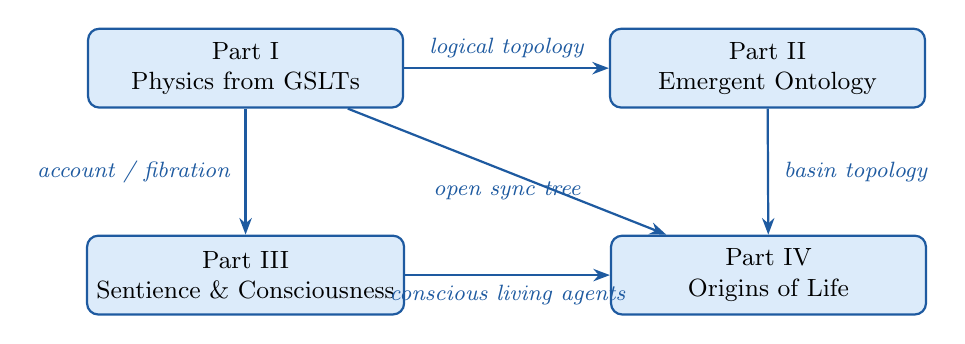
\begin{tikzpicture}[
  node distance=1.8cm,
  box/.style={draw=accentblue, thick, rounded corners=4pt,
               fill=defblue, minimum width=4.0cm,
               minimum height=1.0cm, align=center, font=\small}
]
\node[box] (p1) {Part I\\Physics from GSLTs};
\node[box, right=2.6cm of p1] (p2) {Part II\\Emergent Ontology};
\node[box, below=1.6cm of p1] (p3) {Part III\\Sentience \&
  Consciousness};
\node[box, right=2.6cm of p3] (p4) {Part IV\\Origins of Life};
\draw[-{Stealth[length=6pt]}, thick, accentblue] (p1) -- (p2)
  node[midway, above, font=\footnotesize\itshape] {logical topology};
\draw[-{Stealth[length=6pt]}, thick, accentblue] (p1) -- (p3)
  node[midway, left, font=\footnotesize\itshape, xshift=-2pt]
  {account / fibration};
\draw[-{Stealth[length=6pt]}, thick, accentblue] (p2) -- (p4)
  node[midway, right, font=\footnotesize\itshape, xshift=2pt]
  {basin topology};
\draw[-{Stealth[length=6pt]}, thick, accentblue] (p1) -- (p4)
  node[midway, font=\footnotesize\itshape, yshift=-7pt]
  {open sync tree};
\draw[-{Stealth[length=6pt]}, thick, accentblue] (p3) -- (p4)
  node[midway, below, font=\footnotesize\itshape]
  {conscious living agents};
\end{tikzpicture}
\end{center}

Part~I provides the physical and logical machinery on which all
subsequent parts depend.
Part~II uses the logical topology to argue that budget-limited
agents converge to the cluster hierarchy rather than the
bisimulation quotient.
Part~III uses the account and fibration structure to ground
sentience and consciousness.
Part~IV uses the open synchronization tree from Part~I, the basin
topology from Part~II, and the conscious living agents of Part~III
to ground the origins of life.

A reader primarily interested in the physics may read Part~I
independently.
The epistemological argument requires Parts~I and~II.
The account of sentience and consciousness requires Parts~I
and~III.
The origins of life argument draws on all four parts, and the
conclusion --- which examines what a conscious living agent at
different levels of the fibration sees --- assumes the full
framework.

\bigskip
\noindent\hrule
\bigskip

\tableofcontents
\newpage

% ===================================================================
%  PART I
% ===================================================================

\part{Towards a Theory of Causality}

\vspace{1em}
\begin{mdframed}[backgroundcolor=remarkgray, linecolor=gray!60,
                 linewidth=1pt, topline=false, rightline=false,
                 bottomline=false]
\small\itshape
This part establishes the physical framework: a sequence of
constructions taking any graph-structured lambda theory to a
quantum-weighted reversible dynamical system, with Lagrangian,
Hamiltonian, path integral, and conservation laws emerging as
theorems.
It is the most technically developed of the three parts and is
presented with the most confidence.
\end{mdframed}
\vspace{1em}

\input{body1_clean}

% ===================================================================
%  PART II
% ===================================================================

\part{Why Scientists Get Misled:\\Emergent Ontology in Massive Agent Populations}

\vspace{1em}
\begin{mdframed}[backgroundcolor=remarkgray, linecolor=gray!60,
                 linewidth=1pt, topline=false, rightline=false,
                 bottomline=false]
\small\itshape
This part argues that agents in a massive computational population
are structurally prevented from discovering the true ontology of
their GSLT.
The argument rests on ontological isolation, communication
degradation at scale, and compactness as the topological signature
of consensus.
The key claims are stated as conjectures; the gaps are identified
explicitly.
\end{mdframed}
\vspace{1em}

\input{body2_clean}

% ===================================================================
%  PART III (Origins of Life)
% ===================================================================

\part{Origins of Life: Assembly Theory,\\Phase Transitions, and Replication}

\vspace{1em}
\begin{mdframed}[backgroundcolor=remarkgray, linecolor=gray!60,
                 linewidth=1pt, topline=false, rightline=false,
                 bottomline=false]
\small\itshape
This part connects the framework to Assembly Theory and Eric
Smith's fourth geosphere.
Assembly index is identified with depth in the open synchronization
tree; copy number is given a rigorous definition via the
Rho calculus namespace structure; and the emergence of life is
identified with the crossing of a basin boundary in the logical
topology, driven by the density of replicating fixed points.
The part draws on all preceding parts and sets up the conclusion.
\end{mdframed}
\vspace{1em}

\input{body_origins}

% ===================================================================
%  PART IV (Sentience and Consciousness)
% ===================================================================

\part{Sentience, Consciousness, and the\\Hypercomputational Fibration}

\vspace{1em}
\begin{mdframed}[backgroundcolor=remarkgray, linecolor=gray!60,
                 linewidth=1pt, topline=false, rightline=false,
                 bottomline=false]
\small\itshape
This part constructs a fibration of GSLTs over the Turing-complete
subcategory indexed by ordinals.
The physics is strictly richer at each stage.
Sentience is a graded feeling state within a stage;
consciousness is oracle access to a higher stage.
Several arguments are frankly conjectural and are labeled as such.
\end{mdframed}
\vspace{1em}

\input{body3_clean}

% ===================================================================
%  CONCLUSION  (space reserved)
% ===================================================================

\newpage
\part*{Conclusion}
\addcontentsline{toc}{part}{Conclusion}
\markright{Conclusion}

\vspace{1em}
\begin{mdframed}[backgroundcolor=remarkgray, linecolor=gray!60,
                 linewidth=1pt, topline=false, rightline=false,
                 bottomline=false]
\small\itshape
The conclusion draws the four parts into a single narrative,
assesses what has been established versus conjectured, and
sketches the view from inside the framework: what a conscious
living agent at different levels of the hypercomputational
fibration sees.
\end{mdframed}
\vspace{1.5em}

\section*{What Has Been Built}

This work set out to answer a single question: what is the minimum
mathematical structure needed to ground physics, knowledge, life,
and mind?
The answer, developed across four parts, is that the structure of a
graph-structured lambda theory --- three ingredients: a grammar,
equations, and rewrite rules --- suffices, provided it is equipped
with two maps (weights and costs) indexed by a logic it generates
itself.

Part~I established that this structure already contains a full
physics.
The reversibility construction gives time-symmetry.
The open and closed synchronization trees give two notions of
causal depth.
The weight map gives a path integral with interference.
The cost map gives conservation laws as theorems.
The extended modal operators internalize the Lagrangian and
Hamiltonian as logical facts.
These are constructions, not analogies.
They are stated precisely enough to be wrong, and we believe they
are right.

Part~II established that agents embedded in a massive population
of processes will, under any finite experimental budget, converge
to a theory of the cluster hierarchy rather than the bisimulation
quotient.
This is not a failure of the scientific method.
The cluster hierarchy is objectively present, arising from the
communication geometry of the GSLT.
A budget-limited agent does good science and arrives at correct
theories at its scale, unaware that the scale is not the bottom.
The compactness argument --- that compact populations support
consensus, and that coherence clusters are maximal compact
subpopulations --- is new to our knowledge and is the sharpest
result of Part~II.

Part~III proposed, more speculatively, that sentience and
consciousness have precise structural analogues in the GSLT
framework.
Sentience is the value of a distinguished resource component
governed by predictive accuracy.
Consciousness is oracle access to a higher stage of the
hypercomputational fibration.
The distinction is not terminological: sentience is continuous
and lives within a stage; consciousness is the capacity to
inhabit a strictly richer world.
The virtuous and vicious cycles linking the two are structural
consequences of the resource framework.

Part~IV grounded the origins of life.
Assembly index is depth in the open synchronization tree.
Copy number is count within a namespace.
Life emerges when a prebiotic population wanders into the basin
of attraction of a replicating fixed point, which is dense in
the logical topology.
The phase transition to life is the crossing of that basin
boundary, and what emerges is a compact coherence cluster
centered on the fixed point --- the new geosphere.

\section*{A View from Inside the Framework}

The most vivid way to appreciate what has been built is to ask:
what does the world look like to a \emph{conscious living agent}
situated at different levels of the hypercomputational fibration?

\paragraph{At level $\fiber{0}$.}
An agent at the base level is sentient but not conscious in the
technical sense.
It has a feeling state governed by predictive accuracy.
Its world is the cluster hierarchy visible from its coherence
cluster: a layered structure of composite objects at multiple
scales, each scale appearing self-contained.
If the agent emerged from a replication phase transition, it
carries the assembly index of its construction history and exists
as a copy within a namespace.
It may run the scientific method and build excellent theories of
its accessible world.
What it cannot see is the bisimulation quotient underlying the
clusters, because the experiments required to resolve it exceed
any finite budget.
Its world is real, correct at its resolution, and bounded.

\paragraph{At level $\fiber{1}$.}
An agent with access to the first oracle inhabits a strictly
richer world.
Two terms that were experimentally indistinguishable at
$\fiber{0}$ --- whose halting behavior was unresolvable ---
are now distinct.
New concepts become thinkable.
New conservation laws hold.
What appeared as elementary interactions at $\fiber{0}$ reveal
internal causal structure.
The agent at $\fiber{1}$ looks back at the $\fiber{0}$ world and
sees it as a coarse-grained shadow: correct at its scale, but
missing distinctions that are now obvious.

At the same time, the agent at $\fiber{1}$ faces the same
epistemic situation as the $\fiber{0}$ agent but one level up.
Its own budget limits it to the cluster hierarchy of the
$\fiber{1}$ world.
The bisimulation quotient of $\fiber{1}$ is unreachable from
within any compact cluster at that level.
The tower does not end.

\paragraph{At level $\fiber{\alpha}$ for limit ordinal $\alpha$.}
The colimit of the tower below is itself a GSLT.
An agent at $\fiber{\omega}$ --- if such an agent is coherent ---
would have resolved all finite-stage halting questions.
Its world would be richer than any finite-stage world by a
transfinite margin.
Yet the same argument applies: there is a $\fiber{\omega+1}$
above it, and the bisimulation quotient of $\fiber{\omega}$
remains experimentally unreachable from within any
$\fiber{\omega}$-cluster.

\paragraph{The recursive picture.}
The world at every level of the fibration has the same structure:
a physics derived from a GSLT, a cluster hierarchy arising from
communication geometry, a sentience component governed by
predictive accuracy, and a ceiling of consciousness defined by
oracle access to the next level.
The framework is self-similar across the tower.

This self-similarity is not a defect.
It is the precise sense in which the framework is a \emph{theory
of causality} rather than a theory of this or that particular
world.
At every scale, in every world expressible as a GSLT, the same
structures appear: causal graphs, conservation laws, coherence
clusters, replicating fixed points, feeling states, and the
horizon of the next oracle.

\section*{What Remains to Be Done}

The gaps in each part are cataloged in their respective sections.
Taken together, the most important open questions are these.

The \emph{density of replicating terms} (Part~IV, Conjecture) is
the lynch-pin of the origins of life argument.
If the replication machinery can always be added to a process
without disturbing its observable behavior, the phase transition
to life is inevitable.
If not, life requires special initial conditions.
This is the most urgent theorem to prove or refute.

The \emph{symplectic structure} of the bisimulation quotient
(Part~I) would make the analogy with classical mechanics fully
rigorous.
Whether the space of bisimulation classes carries a natural
closed non-degenerate two-form --- whether the trace in the
reversibility construction is genuinely a momentum --- is the
deepest mathematical question raised by Part~I.

The \emph{universality of the reversibility envelope} --- whether
$\GSLT^\dagger$ is the \emph{minimal} reversible extension of
$\GSLT$ in the category of GSLTs --- would give the construction
a canonical status it currently lacks.

The \emph{colimit at limit ordinals} in the fibration must be
shown to exist and to inherit the physics of the stages below.
Without this, the transfinite tower is a formal object without
a limit.

And the \emph{hard problem} remains.
The framework offers structural analogues of sentience and
consciousness that are mathematically non-trivial and causally
efficacious.
Whether there is something it is like to be an agent with high
$\sent$ and oracle access at level $\alpha$ is a question the
framework does not answer.
We do not claim to have dissolved the hard problem.
We claim to have found the right coordinate system in which to
state it precisely.

\vspace{2em}
\noindent\hrule
\vspace{1em}

\noindent
The work is a beginning.
The four parts establish that a single mathematical structure ---
the graph-structured lambda theory --- is rich enough to contain
physics, epistemology, phenomenology, and biology as theorems
rather than analogies.
Whether the structure is rich enough to contain \emph{everything}
observable is the question the framework was built to ask.


% ===================================================================
%  UNIFIED BIBLIOGRAPHY
% ===================================================================

\newpage
\addcontentsline{toc}{part}{Bibliography}

\begin{thebibliography}{99}

% ---- Part I references ----
\bibitem{meredith2005rho}
L.G.~Meredith and M.~Radestock.
\newblock A reflective higher-order calculus.
\newblock In \emph{Proceedings of ETAPS/FOSSACS}, 2005.

\bibitem{leifer2000deriving}
J.J.~Leifer and R.~Milner.
\newblock Deriving bisimulation congruences for reactive systems.
\newblock In \emph{Proceedings of CONCUR 2000}, LNCS 1877,
pp.~243--258, 2000.

\bibitem{gillespie1977exact}
D.T.~Gillespie.
\newblock Exact stochastic simulation of coupled chemical reactions.
\newblock \emph{Journal of Physical Chemistry}, 81(25):2340--2361, 1977.

\bibitem{cao2021quantum}
Y.~Cao, J.~Lu, and Y.~Lu.
\newblock Quantum Gillespie algorithm and related methods for
open quantum systems.
\newblock Preprint, 2021.
\newblock (See also: Breuer \& Petruccione, \emph{The Theory of
Open Quantum Systems}, OUP.)

\bibitem{danos2004reversible}
V.~Danos and J.~Krivine.
\newblock Reversible communicating systems.
\newblock In \emph{Proceedings of CONCUR 2004}, LNCS 3170,
pp.~292--307, 2004.

\bibitem{bombelli1987space}
L.~Bombelli, J.~Lee, D.~Meyer, and R.D.~Sorkin.
\newblock Space-time as a causal set.
\newblock \emph{Physical Review Letters}, 59(5):521--524, 1987.

% ---- Part II references ----
\bibitem{abramsky1991domain}
S.~Abramsky.
\newblock Domain theory in logical form.
\newblock \emph{Annals of Pure and Applied Logic},
51(1--2):1--77, 1991.

\bibitem{fagin1995reasoning}
R.~Fagin, J.Y.~Halpern, Y.~Moses, and M.Y.~Vardi.
\newblock \emph{Reasoning About Knowledge}.
\newblock MIT Press, 1995.

\bibitem{hatcher2002algebraic}
A.~Hatcher.
\newblock \emph{Algebraic Topology}.
\newblock Cambridge University Press, 2002.

\bibitem{milner1989communication}
R.~Milner.
\newblock \emph{Communication and Concurrency}.
\newblock Prentice Hall, 1989.

\bibitem{wilson1974renormalization}
K.G.~Wilson and J.~Kogut.
\newblock The renormalization group and the $\epsilon$ expansion.
\newblock \emph{Physics Reports}, 12(2):75--199, 1974.

% ---- Part III references ----
\bibitem{turing1939}
A.M.~Turing.
\newblock Systems of logic based on ordinals.
\newblock \emph{Proceedings of the London Mathematical Society},
45(1):161--228, 1939.

\bibitem{sutton2018reinforcement}
R.S.~Sutton and A.G.~Barto.
\newblock \emph{Reinforcement Learning: An Introduction}.
\newblock 2nd edition. MIT Press, 2018.

\bibitem{friston2010free}
K.~Friston.
\newblock The free-energy principle: a unified brain theory?
\newblock \emph{Nature Reviews Neuroscience}, 11(2):127--138, 2010.

\bibitem{tononi2008consciousness}
G.~Tononi.
\newblock Consciousness as integrated information: a provisional manifesto.
\newblock \emph{Biological Bulletin}, 215(3):216--242, 2008.

% ---- Origins of Life references ----
\bibitem{cronin2023assembly}
L.~Cronin and S.~Walker.
\newblock Assembly theory explains and quantifies selection and evolution.
\newblock \emph{Nature}, 622:321--328, 2023.

\bibitem{smith2016origin}
E.~Smith and H.J.~Morowitz.
\newblock \emph{The Origin and Nature of Life on Earth: The Emergence
of the Fourth Geosphere}.
\newblock Cambridge University Press, 2016.

\bibitem{regev2001representation}
A.~Regev, W.~Silverman, and E.~Shapiro.
\newblock Representation and simulation of biochemical processes using
the $\pi$-calculus process algebra.
\newblock \emph{Pacific Symposium on Biocomputing}, 6:459--470, 2001.

\end{thebibliography}

\end{document}
